If we are to require conforming finite elements, Lagrange finite elements are
not enough to guarantee continuity in the first derivative, and so to ensure
continuity in the first derivative \cite{Johnson} a $C^1$ FE will be required.
In this thesis we focus on the Argyris element (depicted in
\autoref{fig:Argyris}), although the FE error analysis presented in
\autoref{sec:QGEError}, \autoref{sec:SQGEErrors}, and \autoref{sse:SQGE2LE} only
requires the use of a $C^1$ FE. The Argyris element is probably the best known
of all $C^1$ finite elements \cite{Argyris,Dominguez08}, but appears to be rarely
implemented.

\begin{figure}[h]
	\begin{center}
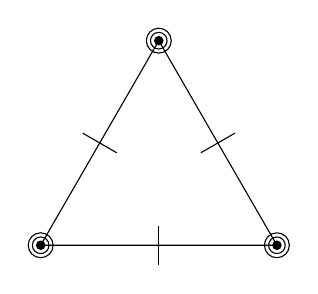
\begin{tikzpicture}[scale=0.5]
	%define the vertices of the triangle
	\path[coordinate] (0,0) coordinate(A)
		++(60:3cm) coordinate(D)
		++(60:3cm) coordinate(B)
		++(-60:3cm) coordinate(E)
		++(-60:3cm) coordinate(C)
		++(180:3cm) coordinate(F);
	%label the vertices and draw edges
	\draw (A) -- (D) -- (B) -- (E) -- (C) -- (F) -- cycle;
	%draw the interpolation points
	%function values
	\filldraw[black] (A) circle(3pt); 
	\filldraw[black] (B) circle(3pt); 
	\filldraw[black] (C) circle(3pt); 
	%first derivatives
	\draw[black] (A) circle(6pt); 
	\draw[black] (B) circle(6pt); 
	\draw[black] (C) circle(6pt); 
	%second derivatives
	\draw[black] (A) circle(9pt); 
	\draw[black] (B) circle(9pt); 
	\draw[black] (C) circle(9pt); 
	%normal derivatives
	\draw (1.067,2.848) -- (D) -- (1.933,2.348); 
	\draw (4.067,2.348) -- (E) -- (4.933,2.848); 
	\draw (3,-0.5cm) -- (F) -- (3,0.5cm); 
	%labels
%	\node[below of=A, node distance=0.5cm] (k) {$k=j+1$};
% \node[above of=B, node distance=0.5cm] (j) {$j=i+1$};
%	\node[below of=C, node distance=0.5cm] (i) {$i$};
\end{tikzpicture}
	\end{center}
	\caption{Argyris element with its 21 degrees of freedom.}
	\label{fig:Argyris}
\end{figure}


The Argyris element does, in fact, ensure $C^1$ continuity
\cite{Dominguez08,Okabe}, but at a cost of twenty-one degrees of freedom.
However, these twenty-one degrees of freedom give basis polynomials of degree
five and therefore the FE discretization with the Argyris element has a high
rate of convergence \cite{Dominguez08}.  These degrees of freedom include the
value at each vertex, the value of the first derivatives at each vertex, the
value of the second derivatives at each vertex, the value of the mixed
derivative at each vertex, and finally the value of the normal derivatives at
each of the edge midpoints. Here in lies the main difficulty in implementing the
Argyris triangle, the normal derivatives. Not only do we now have 21 degrees of
freedom that we must worry about, but the added complexity of a transformation
that maintains the direction of the normal derivatives is required. Since
working on the reference element is the most common way of working with finite
elements and normal derivatives are not respected by affine transformation a
more complicated transformation will have to be employed. This is unlike a
standard Lagrange element where only a simple affine transformation is required
\cite{Dominguez08}.

Dominguez \emph{et al.} developed such a transformation. This transformation,
which is a $21 \times 21$ matrix, $C$, allows for all calculations to be done on
a reference element \cite{Dominguez08}, vastly simplifying the calculations for
the various matrices and load vector required for the QGE finite elements
calculations and allowing for faster running code. Since the tranformation
developed by Dominguez is so new, and is not the standard for implementation of
the Argyris element, his transformation will be discussed at length in
\autoref{sse:Trans} for completeness.
